
\documentclass[
  aspectratio=1610, 
  xcolor={dvipsnames},
  % handout
]{beamer}

\usetheme{metropolis}

\setbeamercolor{background canvas}{bg = white}

% macro.tex

\usepackage{graphicx}
\usepackage{amsmath}
\usepackage{multicol}
\usepackage{tabularx}
\usepackage{array}
\newcolumntype{x}[1]{>{\centering\arraybackslash\hspace{0pt}}p{#1}}
% \setlength{\columnseprule}{1pt}
% \def\columnseprulecolor{\color{block body.fg}}
\usepackage{tikz, pgfplots}
\usetikzlibrary{shapes.geometric, shapes, fit, arrows, calc, fit, positioning, chains, arrows.meta, backgrounds, calc}

% subject specific
\usepackage{amsmath, amssymb}

% drawing
\usepackage{pstricks}
\usepackage{tikz, tkz-orm, pgfplots}
\usetikzlibrary{arrows,shapes,backgrounds,decorations.markings}
\usetikzlibrary{matrix,positioning,decorations.pathreplacing,calc,tikzmark}
\pgfplotsset{width=7.5cm,compat=1.16}
\usepgfplotslibrary{fillbetween}

% listings
\usepackage[final]{listings}
% \usepackage{unicode-math}
% \usepackage{xunicode}
% \usepackage{fontspec}
% \setmonofont[
%   Contextuals={Alternate}
% ]{Fira Code}

\definecolor{codegreen}{rgb}{0,0.6,0}
\definecolor{codegray}{rgb}{0.5,0.5,0.5}
\definecolor{codepurple}{rgb}{0.58,0,0.82}
\definecolor{backcolour}{rgb}{1,1,1}

\lstdefinestyle{stolenstyle}{
    backgroundcolor=\color{backcolour},
    commentstyle=\color{codegreen},
    keywordstyle=\color{magenta},
    numberstyle=\tiny\color{codegray},
    stringstyle=\color{codepurple},
    basicstyle=\ttfamily\footnotesize,
    breakatwhitespace=false,
    breaklines=true,
    captionpos=b,
    keepspaces=true,
    numbers=left,
    numbersep=5pt,
    showspaces=false,
    showstringspaces=false,
    showtabs=false,
    tabsize=2,
    inputencoding=utf8,
    extendedchars=true,
    language=scala,
    % texcl=false,
    mathescape=false,
    % escapechar=\&,
    literate = 
        {=>}{{=>}} {2}
        {->}{{->}} {2}
        {_}{{\_}} {1}
        {|}{\textbar} {1}
        {==>}{{==>}} {3},
}

\lstset{style=stolenstyle}

\lstdefinestyle{lisa}{
    backgroundcolor=\color{backcolour},   
    commentstyle=\color{codegreen},
    keywordstyle=\color{magenta},
    numberstyle=\tiny\color{codegray},
    stringstyle=\color{codepurple},
    basicstyle=\linespread{1.4}\ttfamily\footnotesize,
    breakatwhitespace=false,         
    breaklines=false,                 
    captionpos=b,                    
    keepspaces=true,                 
    numbers=left,                    
    numbersep=5pt,                  
    showspaces=false,                
    showstringspaces=false,
    showtabs=false,                  
    tabsize=2,
    keywordstyle = [2]{\color{OliveGreen}},
    keywordstyle = [3]{\color{Blue}},
    keywordstyle = [4]{\color{BrickRed}},
    morekeywords = [2]{val, Theorem, have, thenHave, andThen, by},
    morekeywords = [3]{AccOutNil},
    morekeywords = [4]{Apply},
    literate = 
        {===}{{===}} 3
        {::}{{::}}   2
        {->}{{->}}   2,
}

% \lstset{style=lisa}

% links and citations
\usepackage{hyperref, bookmark}
\hypersetup{hidelinks} % hide boxes around links ew
% pls add color
\usepackage{csquotes}
% \usepackage{polyglossia}
% \setdefaultlanguage{english}
\usepackage[
    style=numeric,
    sorting=none,
    maxnames=99,
    language=english
]{biblatex}
\addbibresource{biblio.bib}

\usepackage{mathpartir}
\usepackage{stmaryrd}

\newcommand{\mathcomment}[1]{\text{\textcolor{black!50}{\emph{#1}}}}


\title{Are bananas a good source of recursion in your diet?}
\author{Sankalp Gambhir}

\begin{document}

\maketitle

\begin{frame}
  \frametitle{Reference}

  Main reference: 

  \fullcite{meijer1991functional}

  But also:

  \fullcite{nlab:recursion_scheme}

  \fullcite{wiki:falgebra}

  \fullcite{milewski2019category}

\end{frame}

% goto
% for/while
\begin{frame}[fragile]
  \frametitle{Back to basics}

  \begin{lstlisting}(language=C++)
int fac(int target) {
  int i = 1;
  int n = 1;
  
  start:
    if (n > target) goto end;
    i *= n++;
    goto start;
  end:
  
  return i;
}
  \end{lstlisting}

  % while the structure of jumps here is not complex, it is made obscure by its
  % ad hoc nature, and in almost all scenarios today, we would frown upon this 
  % implmentation

  % instead opting for something like this

\end{frame}

\begin{frame}[fragile]
  \frametitle{Abstracting out of shame}

  \begin{lstlisting}(language=C++)
int facw(int target) {
  int i = 1;
  int n = 1;
  
  while (n <= target) i *= n++;
  
  return i;
}
  \end{lstlisting}  

  % the structure of the loop is now clearer, the code is more readable,
  % significantly smaller, and will unfold to practically the same thing

\end{frame}

% recursion
\begin{frame}[fragile]
  \frametitle{Shamelessly recursive}

  % recursive program
  \begin{lstlisting}{language=scala}
def facr(target: Int): Int = 
  if target <= 0 then 
    1 
  else 
    target * facr(target - 1)
\end{lstlisting}

  % it's certainly convenient, captures the essence of the problem well but the
  % recursion is still ad hoc, it can be non-linear, it's non-tail recursive,
  % the termination is not obvious

  % while better than the imperative versions, we can do better, of course
  \pause

\begin{lstlisting}{language=scala}
def facf(target: Int): Int = 
  (1 to target).fold(1)(_ * _)
\end{lstlisting}

\end{frame}

% why do we not apply the same level of scrutiny to arbitrary recursion?
% we do, already, in a sense, use abstractions over recursion often
% <interactive> list functions people like to use, keep it somewhat minimal

\begin{frame}
  \frametitle{What can we do with our abstractions?}

  \begin{itemize}[<+->]
    \item \lstinline|goto| can express any computable function
    \item So can \lstinline|while| loops
    \item What about recursion v our abstractions? Is there a subset that allows
    expressing a reasonably large set of functions? All the recursively
    computable functions?
  \end{itemize}

  % and disclaimer, I don't have a perfect concrete answer to present, but
  % that's the general problem we are interested in rn 

\end{frame}

% introduce catamorphisms over lists
% fold is exactly a catamorphism
% what other things fit in?
% clearly not all
\begin{frame}[fragile]
  \frametitle{Catamorphism}

  ``Cata'' - down/downwards \vspace{3em}

  \pause

  \begin{lstlisting}
def cataList[A, B](b: B)(*: (A, B) => B)(l: List[A]): B =
  l match {
    case Nil => b
    case h :: t => h * cataList(b)(f)(t)
  }
  \end{lstlisting}

  % well, the structure looks familiar
  % it's a fold

  % but, makes sense, we are destructing a list going top-down, 
  % and accumulating a result

  \pause

  Given a \lstinline|b : B|, a function \lstinline|*: (A, B) => B|, \((\mspace{-5mu}|\)\lstinline|b|, \lstinline|*|\(|\mspace{-5mu})\)
  is a catamorphism over lists of type \lstinline|A|. The final type is \lstinline|List[A] => B|.

  % so, which of our functions fit into this type?

  % well, there are clearly still recursive functions over lists that don't fit
  % into this bucket 

  % so we had list a to b, let's consider the *converse*. Given some data b, can
  % we constructively produce a list a?

\end{frame}

% anamorphisms

\begin{frame}[fragile]
  \frametitle{Anamorphism}

  ``Ana'' - up/upwards \vspace{3em}

  \pause

  \begin{lstlisting}
def cataList[A, B](b: B)(*: (A, B) => B)(l: List[A]): B =
  l match {
    case Nil => b
    case h :: t => h * cataList(b)(f)(t)
  }
  \end{lstlisting}

  \pause
  \begin{itemize}[<+->]
    \item stopping point / base case
    \item inductive case - a way to split a \lstinline|B| into an \lstinline|h|
    and a \lstinline|t|. \pause Sufficient to have an \lstinline|h| and a
    \lstinline|b1|.
  \end{itemize}

\end{frame}

\begin{frame}[fragile]
  \frametitle{Anamorphism}

  ``Ana'' - up/upwards \vspace{3em}

  \pause

  \begin{lstlisting}
def anaList[A, B](p: B => Bool)(g: B => (A, B))(b: B): List[A] =
  if p(b) then 
    Nil 
  else
    val (h, b1) = g(b)
    h :: anaList(p)(f)(b1)
  \end{lstlisting}

  or an \emph{`unfold'}. Written as concave lenses \([\mspace{-5mu}(g, p)\mspace{-5mu}]\).

  % what things fit in here?

\end{frame}

% hylomorphisms

\begin{frame}[fragile]
  \frametitle{Hylomorphism}

  Look back at \lstinline|facf|

\begin{lstlisting}
def facf(target: Int): Int = 
  (1 to target).fold(1)(_ * _)
\end{lstlisting}

  \pause We produce a list (ana) and then immediately consume it (cata). \pause
  The composition of an anamorphism (\lstinline|B => List[A]|) and a catamorphism
  (\lstinline|List[A] => C|) is a \emph{hylomorphism}.

  \pause
  `Hylo' - `dust/matter' (wood?). Originating from philosophical idea that form and
  matter are one. Written \([\mspace{-3mu}[(b, *), (g, p)]\mspace{-3mu}]\).

\end{frame}

% relation to tail recursion

\begin{frame}
  \frametitle{Hylomorphisms, in principle}

  The list was not necessary in the computation, we just used it as a concrete
  data representation of our computation plan. \pause In the end, the
  computation was on a completely different data type (nat)! \pause
  
  Hylomorphisms are more generally any functions whose call trees are
  ``list-like''. \pause (I think these are exactly linear recursive functions?)

\end{frame}

% ok, all well known facts, but with a different name
% so why are we here

% there are two main things we would like to 
% understand about catamorphisms

\begin{frame}
  Why are we reiterating this with different names and pretty frames? \pause

  Why? \pause Why these abstractions? 

\end{frame}

% cata as unique morphism from initial F algebra
% cata as the haskell def
\begin{frame}[fragile]
  \frametitle{Downward into catamorphisms}

  \pause
  \begin{quote}
    A catamorphism (a.k.a. a fold) is the unique F-algebra homomorphism from an
    initial algebra for the functor \(F\).
  \end{quote}
    \pause Or:
  \begin{quote}
    Given an endofunctor F such that the category of F-algebras has an initial
    object \((\mu F,in)\), the catamorphism for an F-algebra \((A,\varphi)\) is the unique
    homomorphism from the initial F-algebra \((\mu F,in)\) to \((A,\varphi)\). The unique
    morphism between the carriers is also denoted \(cata~ \varphi: \mu F \to A\).
  \end{quote}

  \pause
  Or in code:
  \begin{lstlisting}
    cata :: Functor f => Algebra f a -> Fix f -> a
    cata alg = alg . fmap (cata alg) . unfix
  \end{lstlisting}

  \pause
  This one line describes \emph{all} folds. Not over lists, not over trees, but
  \emph{all possible} folds.

\end{frame}

% what do these two mean at all? 

\begin{frame}
  \frametitle{Just Enough Category Theory to be Dangerous}

  A \emph{category} is a collection of objects (points) and a collection of
  morphisms (arrows) between them. 

  \begin{itemize}
    \item For every object \(A\), there is an identity morphism \(id_A: A \to A\)
    \item If \(f: A \to B\) and \(g: B \to C\), there must be a morphism \(h: A
    \to C\) such that \(g \circ f = h\).
    \item Composition is associative.
  \end{itemize}

  \begin{center}
    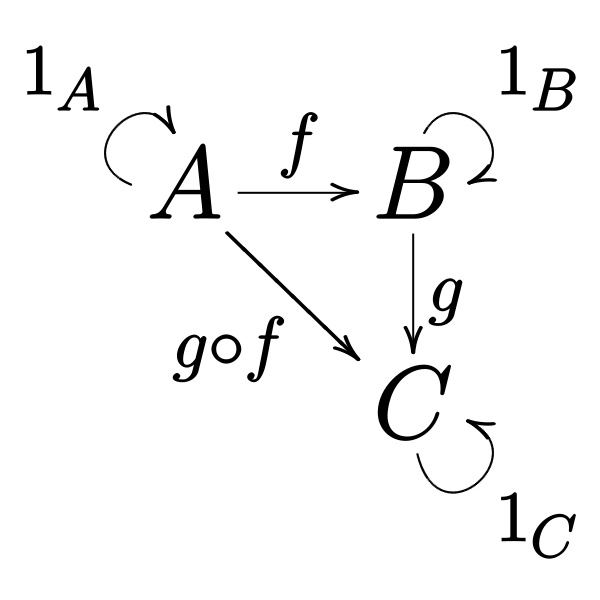
\includegraphics[height = 8em]{fig/cat.png}
  \end{center}

\end{frame}

\begin{frame}
  \frametitle{Just Enough Category Theory to be Dangerous}

  A \emph{functor} is a mapping between categories that preserves the structure
  of the category.
  
  \begin{itemize}
    \item For every object \(A\), there is a corresponding object \(F(A)\).
    \item For every morphism \(f: A \to B\), there is a morphism \(F(f): F(A)
    \to F(B)\).
    \item Identity is preserved: \(F(id_A) = id_{F(A)}\).
    \item Composition is preserved: \(F(g \circ f) = F(g) \circ F(f)\).
  \end{itemize}
  
  \begin{center}
    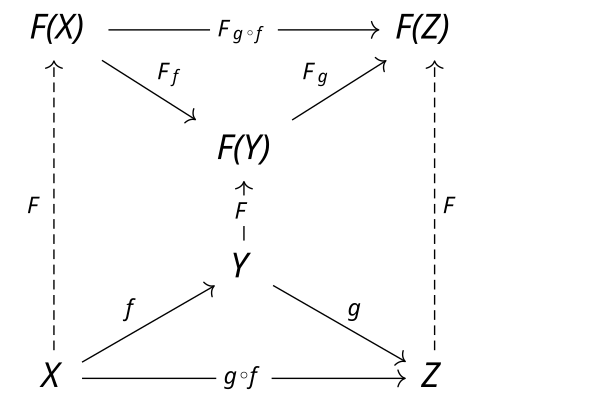
\includegraphics[height = 11em]{fig/fun.png}
  \end{center}

\end{frame}

\begin{frame}
  \frametitle{Just Enough Category Theory to be Dangerous}

  We are mostly interested in \emph{endofunctors} on types, i.e. functors that
  map some category containing types from our program to itself, mapping some
  types to other types, and correspondingly their functions.

  \pause
  For example, \lstinline|List[_]| is a functor (\lstinline|Type =>> Type|) that
  maps any type \lstinline|A| to \lstinline|List[A]|, and a function
  \lstinline|A => B| to a function \lstinline|List[A] => List[B]|.

\end{frame}

\begin{frame}

  Missing \emph{initial}, \emph{F-algebra}, and related terms. Hopefully
  understood better through code.

  \begin{center}
    \Huge Implementation
  \end{center}

\end{frame}

% <live code>

% what is an algebra?
% what is an initial algebra?
\begin{frame}
  \frametitle{Algebra}

  For an endofunctor \(F\) on a category \(C\), an \(F\)-algebra is a pair \((A,
  \alpha)\) where \(A\) is an object in \(C\) and \(\alpha: F(A) \to A\) is a
  morphism in \(C\).

  \pause

  So \((A, \alpha)\) can be an algebra if and only if there is a way to reduce
  values of the "next iteration" of \(F\) back into \(A\), i.e., \(A\) is closed
  under \(F(\cdot)\) (by \(\alpha\)).
  
  \pause

  We can check that these algebras form a category with algebra homomorphisms as
  their morphisms. This category has an \emph{initial object}, which is a bit
  like the bottom element in a lattice, it has an arrow to every other object in
  the category.

  So we are saying, an initial algebra can be `embedded' (via a homomorphism) into
  all other algebras. It is a minimal F-algebra. 

  In particular, we used the fact that our language, the meta-logic, has a way
  to provide us least fixpoint semantics (via recursive type definitions), so
  the result is in fact the least fixpoint of the functor.

\end{frame}

% what is a catamorphism?
% write the def
% what do each of these individual things even do?
% we have started from a shallow functor for a datatype
% and derived a general recursion principle
% there is not much here that we did not know, in practical terms
% but there is a certain beauty to the process

% Till last week, I could understand all of the words here individually, but
% make no sense of the whole sentence. Today, I have sort of crossed the barrier
% just enough to understand what this says and start experimenting with it

\begin{frame}
  \frametitle{Why am I looking at recursion schemes?}

  \begin{itemize}
    \item Well, it's interesting. What constructs do we finally really need to
    eliminate arbitrary recursion?
    \item What kind of analysis can we do on programs when we know they are
    composed of only these schemes?
    \item Existing work on decidable verification of programs with catamorphisms
    as theory extensions. Led to the questions "why catamorphisms?" and "what
    more is out there?"
    \item Once we (I) understand catamorphisms, the next thing to understand is
    why they lead to decidable theories. 
    \item How do structured recursion schemes relate to other decidable
    fragments, e.g. sufficiently surjective functions, which (I think) subsume
    catamorphisms? 
  \end{itemize}

  All good questions to hopefully answer in the next few lifetimes.

\end{frame}

\begin{frame}

  \begin{center}
    \Huge Thank you!
  \end{center}

\end{frame}

% we will hopefully understand and come back to conjugate hylomorphisms at some
% point

% open questions and motivations
%% we kinda know while loops can emulate more or less what goto did, in practice
%% what is the analogue for recursion? 
%% there are clearly non catamorphic functions
%% what about non cata/ana/hylomorphisms?
%% can we represent partial functions (sometimes non terminating)? should we?

%% questions for my research
%% what kind of recursive schemes can we efficiently verify?
%% we know that Horn clauses over datatypes + catamorphisms are doable (kinda)
%% other classifications (sufficiently surjective (Suter / Dotta / Kuncak))

\end{document}
